\documentclass{article}
\usepackage[utf8]{inputenc}
\usepackage{graphicx}

\author{Bijan Varjavand}
\title{LabNotebook}
\date{February 21, 2017}

\begin{document}

\maketitle

\section{Objectives}

The goal this lab was to measure capacitance values using an LCR meter, using the results to confirm equations covered in class.

\section{Setup}

LCR meters and the materials were provided by the lab. We were also given copper tape.
\subsection{Materials}

We specifically look at inorganic materials and polymers. Ceramic, firebrick, and glass.
\subsection{Tools}

We used LCR meters and wires along with alligator clips.
\section{Procedure}

We made 3 different copper tape sizes, attaching them to either side of our materials (9 total). Then, contacting opposite sided probes, measured capacitance. We took the results of capacitance from the LCR meters, making sure to note the units in each measurement. Additionally, the dissipation factor was measured. This was done for 3 different frequencies: 100Hz, 1kHz, 100kHz.

\section{Results}

An example of the trends we found from these measurements are shown below.

\begin{figure}[h!]
\centering
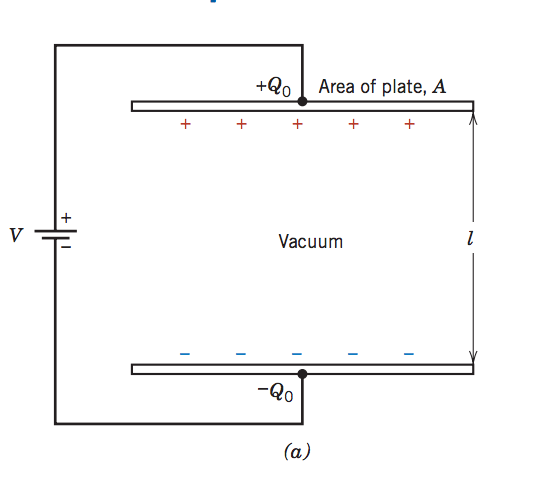
\includegraphics[scale=0.7]{cap.png}
\end{figure}

\section{Observations}

The equations we went over in class were confirmed, namely the fact that capacitance is proportional to the surface area of the copper tape. We also see that the dielectric constant of each of our materials are different, as characterized by the slopes of the above graph.

\end{document}